\bibliographystyle{babplain-fl}

\chapter{Máxima subsecuencia común, otra mirada}
\label{cha:LCS-practical}

  Discutimos el problema de máxima subsecuencia común
  (LCS,
   por el inglés \emph{\foreignlanguage{english}{Longest Common Subsequence}})
  dando algoritmos basados en programación dinámica
  (sección~\ref{sec:LCS},
   el algoritmo de Wagner-Fischer~%
     \cite{wagner74:_string_string_correc_probl},
   aunque Navarro~%
     \cite{navarro01:_guided_tour_approx_strin_match}
   halla múltiples autores independientes de la misma idea)
  y las variantes de Hirschberg~%
    \cite{hirschberg75:_linear_space_algor_comput_maxim_common_subseq}
  para ahorrar espacio
  (discutido en la sección~\ref{sec:ahorrar-espacio}).
  Otros algoritmos para este problema incluyen el de Hunt-Szymanski~%
    \cite{hunt77:_fast_algor_comput_lcs}.
  Una visión distinta es la de Heckel~%
    \cite{heckel78:_techn_isolat_differ_between_files},
  quien intenta reconstruir diferencias fijándose en líneas únicas
  en ambos archivos,
  con el objetivo de obtener diferencias intuitivamente relevantes.
  Una discusión bastante completa de diferentes algoritmos
  es la de Hirschberg~%
    \cite{hirschberg97:_serial_comp_distances}.
  Aho, Hirschberg y Ullman~%
    \cite{aho76:_bound_compl_longes_common_subseq_probl}
  derivan cotas inferiores para el problema general,
  concluyen que en caso de solo comparar símbolos por igualdad
  y alfabeto ilimitado
  (la situación de comparar archivos,
   donde una línea representada por un \emph{\foreignlanguage{english}{hash}}
   es un símbolo)
  en el caso general comparar dos secuencias de largo \(N\)
  demanda tiempo \(\Omega(N^2)\).

  El problema halla aplicación práctica en muchas áreas,
  prominente en las cuales es comparar archivos
  (como describen Hunt y McIllroy~%
    \cite{hunt76:_algor_differ_file_compar}
   y Miller y Myers~%
    \cite{miller85:_file_compar_progr}).
  Los sistemas de control de versiones
  deben mostrar diferencias entre archivos de diferentes versiones,
  y muchos usan internamente las diferencias entre versiones
  para ahorrar espacio al almacenar la historia.
  Ejemplos tempranos son SCCS~%
    \cite{rochkind75:_sccs}
  y RCS~%
    \cite{tichy85:_rcs}.
  Claro que en esta aplicación
  (y al comprimir datos)
  se suele usar además la idea de hacer referencia a copias anteriores
  de los mismos datos.
  El algoritmo básico es de Bentley y McIllroy~%
    \cite{bentley99:_data_compr_using_long_common_strin},
  se estandarizó en el formato VCDIFF~%
    \cite{rfc3284}
  y hay herramientas código abierto,
  como \lstinline[language =]{xdelta}~%
    \cite{macdonald16:_xdelta}.

  Para aplicaciones prácticas
  (archivos de muchos miles de líneas,
   secuencias de genes de muchos millones de pares de bases)
  los algoritmos presentados no son adecuados.
  Hunt y McIllroy~%
    \cite{hunt76:_algor_differ_file_compar}
  comparan algunas alternativas tempranas,
  y plantean técnicas para mejorar el rendimiento,
  como usar un \emph{\foreignlanguage{english}{hash}}
  (ver el capítulo~\ref{cha:hashing} para la teoría del caso)
  en vez de la línea completa para acelerar las comparaciones y ahorrar espacio
  (esto es usar huellas digitales,
   tema que discutiremos en el capítulo~\ref{cha:randomized-algorithms}).
  Concluyen que los algoritmos disponibles en ese entonces
  no hacen diferencia para los casos a su alcance
  (archivos de \num{3\,500}~líneas),
  el tiempo de ejecución está dominado por la lectura de los datos
  y manipulación de caracteres individuales.
  Advertimos,
  eso sí,
  que los distintos algoritmos tienen comportamientos diferentes,
  no siempre este es el más adecuado.
  Barabucci et al~%
    \cite{barabucci16:_measur_qualit_diff_algor}
  discuten varios escenarios e intentan formalizar \textquote{calidad}
  aplicada específicamente a diferencias entre documentos en XML.

  Hoy el algoritmo empleado con mayor frecuencia
  es el de Myers~%
    \cite{myers86:_O_n_d_differ_algor_its_variat},
  cuya variante debida a Wu, Manber, Myers y Miller~%
    \cite{wu90:_sequence_comparison_algorithm}
  discutiremos a continuación.
  Bergroth, Hakonen y Raita~%
    \cite{bergroth00:_survey_longes_common_subseq_algor}
  comparan varios algoritmos,
  para situaciones en las cuales las secuencias son similares
  este algoritmo parece ser el mejor.

  Suponemos dos textos,
  \(X\) e \(Y\),
  de largos \(M = \lvert X \rvert\)
  y \(N = \lvert Y \rvert\),
  donde sin pérdida de generalidad asumimos \(N \ge M\),
  con subsecuencia común máxima de largo \(L\).
  La diferencia entre los largos es \(\Delta = N - M\).
  Sea \(D = M + N - 2 L\),
  el largo de la secuencia de edición
  (operaciones agregar/eliminar)
  más corta
  (de \(X\) debemos eliminar \(M - L\)~símbolos,
   luego hay que insertar \(N - L\) para crear \(Y\)).
  A este valor se le llama \emph{distancia de Levenshtein}~%
    \cite{levenshtein66:_binar_codes_capab_correc_delet_inser_rever}.
  Una medida relacionada,
  que llamaremos \(P\),
  es el número de símbolos eliminados de \(X\):
  \begin{align*}
    P
      &= M - L \\
      &= M - \frac{M + N - D}{2} \\
      &= \frac{D - \Delta}{2}
  \end{align*}
  El algoritmo planteado tiene tiempo de ejecución \(O(N P)\),
  lo que lo hace aplicable
  en situaciones comunes en que las palabras a comparar
  son muy similares.
  Se basa en una formulación intuitiva de grafo de edición,
  es un algoritmo de programación dinámica
  que aprovecha un criterio voraz para limitar las opciones a considerar.

\section{Grafo de edición}
\label{sec:grafo-edicion}

  Sean palabras \(X = x_1 x_2 \ldots x_M\)
  e \(Y = y_1 y_2 \ldots y_N\),
  de largos respectivos \(M\) y \(N\) con \(N \ge M\).
  El \emph{grafo de edición}
  para \(X\) e \(Y\) tiene nodos en los puntos de la cuadrícula
  \((i, j)\) para \(0 \le i \le M\) y \(0 \le j \le N\).
  Los nodos se conectan mediante arcos dirigidos
  verticales, horizontales y diagonales,
  formando un grafo dirigido acíclico.
  Arcos horizontales conectan \((i - 1, j)\) con \((i, j)\),
  arcos verticales conectan \((i, j - 1)\) con \((i, j)\),
  hay un arco diagonal \((i - 1, j - 1)\) a \((i, j)\)
  siempre que \(x_i = y_j\).
  Nuestro problema es llegar desde la \emph{fuente} \((0, 0)\)
  al \emph{sumidero} \((M, N)\) en este grafo.
  Un camino más corto usará el máximo posible de pasos diagonales,
  nos da la subsecuencia común más larga.
  Nuestra medida de distancia es el número de eliminaciones en \(X\),
  que corresponden a pasos verticales.
  La figura~\ref{fig:grafo-edicion} ilustra este grafo
  para \(X = a c b d e a c b e d\)
  e \(Y = a c e b d a b b a b e d\),
  ejemplo de~%
    \cite{wu90:_sequence_comparison_algorithm}.
  \begin{figure}[ht]
    \centering
    \tikzstyle{vertex} = [circle, inner sep = 0pt, minimum size = 0.7mm, fill]
    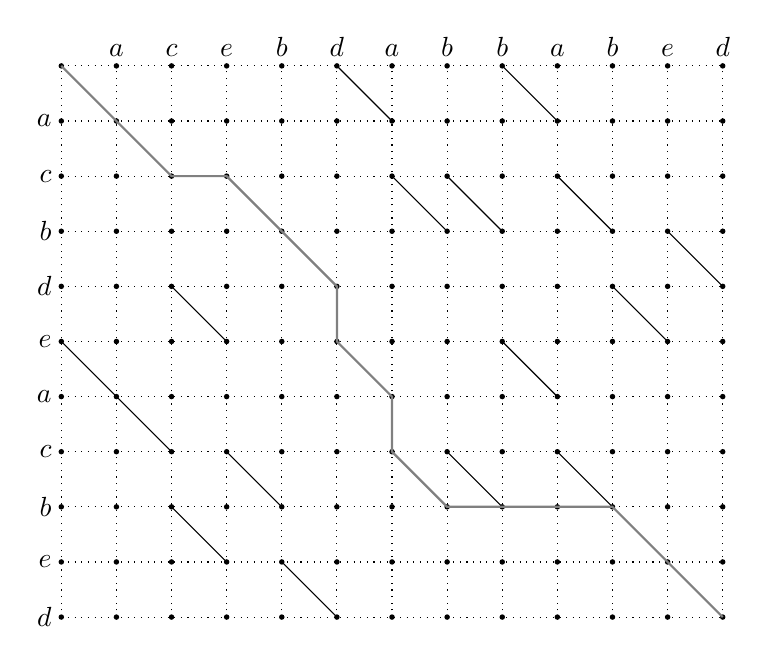
\begin{tikzpicture}[scale = 0.7]
      \foreach \i in {0, 1, ..., 12}
      {
        \foreach \j in {0, 1, ..., 10}
        {
          \node[vertex] at (\i, \j) {};
        }
      }
      \foreach \i in {0, 1, ..., 12}
      {
        \draw[dotted] (\i, 0) -- (\i, 10);
      }
      \foreach \j in {0, 1, ..., 10}
      {
        \draw[dotted] (0, \j) -- (12, \j);
      }

      % Y = acebdabbabed
      \node at ( 1, 10) [above] {\(a\)};
      \node at ( 2, 10) [above] {\(c\)};
      \node at ( 3, 10) [above] {\(e\)};
      \node at ( 4, 10) [above] {\(b\)};
      \node at ( 5, 10) [above] {\(d\)};
      \node at ( 6, 10) [above] {\(a\)};
      \node at ( 7, 10) [above] {\(b\)};
      \node at ( 8, 10) [above] {\(b\)};
      \node at ( 9, 10) [above] {\(a\)};
      \node at (10, 10) [above] {\(b\)};
      \node at (11, 10) [above] {\(e\)};
      \node at (12, 10) [above] {\(d\)};
      % X = acbdeacbed
      \node at (0, 9) [left] {\(a\)};
      \node at (0, 8) [left] {\(c\)};
      \node at (0, 7) [left] {\(b\)};
      \node at (0, 6) [left] {\(d\)};
      \node at (0, 5) [left] {\(e\)};
      \node at (0, 4) [left] {\(a\)};
      \node at (0, 3) [left] {\(c\)};
      \node at (0, 2) [left] {\(b\)};
      \node at (0, 1) [left] {\(e\)};
      \node at (0, 0) [left] {\(d\)};
      % Diagonals
      \draw[thin] ( 0,	5) -- ( 2, 3);
      \draw[thin] ( 2,	6) -- ( 3, 5);
      \draw[thin] ( 2,	2) -- ( 3, 1);
      \draw[thin] ( 3,	3) -- ( 4, 2);
      \draw[thin] ( 4,	1) -- ( 5, 0);
      \draw[thin] ( 5, 10) -- ( 6, 9);
      \draw[thin] ( 6,	8) -- ( 7, 7);
      \draw[thin] ( 7,	8) -- ( 8, 7);
      \draw[thin] ( 7,	3) -- ( 8, 2);
      \draw[thin] ( 8, 10) -- ( 9, 9);
      \draw[thin] ( 8,	5) -- ( 9, 4);
      \draw[thin] ( 9,	8) -- (10, 7);
      \draw[thin] ( 9,	3) -- (10, 2);
      \draw[thin] (10,	6) -- (11, 5);
      \draw[thin] (11,	7) -- (12, 6);
      % A shortest path
      \draw[thick, gray] (0, 10) -- (2, 8) -- (3, 8) -- (5, 6) -- (5, 5)
                           -- (6, 4) -- (6, 3) -- (7, 2) -- (10, 2) -- (12, 0);
    \end{tikzpicture}
    \caption{Un grafo de edición y un camino óptimo}
    \label{fig:grafo-edicion}
  \end{figure}
  En la figura~\ref{fig:grafo-edicion}
  se remarca un camino de \((0, 0)\) a \((12, 10)\),
  correspondiente a
  \(a c b d a b e d
      = x_1 x_2 x_4 x_5 x_6 x_7 x_{11} x_{12}
      = y_1 y_2 y_3 y_4 y_6 y_8 y_9 y_{10}\).
  Una movida vertical corresponde a eliminar un símbolo de \(X\),
  una horizontal inserta un símbolo de \(Y\),
  un paso diagonal es retener el símbolo de ambos
  (parte del camino común más largo).
  En este ejemplo hay \(P = 2\) eliminaciones de \(X\)
  y un total de \(D = 6\) ediciones,
  la secuencia común más larga es de \(L = 8\).
  Hay caminos más cortos alternativos,
  como se ven en la figura~\ref{fig:grafo-edicion}.

\section{Preliminares}
\label{sec:LCS-WMMM:preliminares}

  Considere el grafo de edición dibujado como grilla.
  Sea la diagonal \(k\)
  los puntos \((i, j)\) tales que \(i - j = k\).
  La fuente está sobre la diagonal \num{0},
  el sumidero sobre la diagonal \(\Delta = N - M\).
  Tenemos diagonales numeradas \(-M\) a \(N\).
  El algoritmo presente considera los nodos en la franja de diagonales
  entre \(-P\) y \(\Delta + P\).
  Esto porque todo camino que salga de esta franja
  incluye más de \(P\) pasos verticales:
  si pasa por un vértice bajo \(-P\),
  para llegar a él desde la fuente da más de \(P\) pasos verticales;
  si pasa por un vértice sobre \(\Delta + P\)
  requiere más de \(P\) pasos para llegar al sumidero.

  La \emph{distancia de edición} a \((i, j)\),
  anotada \(D(i, j)\),
  es el costo
  (número total de inserciones y eliminaciones)
  de un camino óptimo de \((0, 0)\) a \((i, j)\)
  sobre la diagonal \(k = i - j\).
  Si tal camino contiene \(v\) pasos verticales y \(h\) horizontales,
  el número de pasos no diagonales es \(v + h = D(i, j)\),
  y debe terminar en la diagonal \(h - v = k\).
  El número de pasos verticales,
  \(V(i, j)\),
  en este camino es una cantidad bien definida:
  es \(V(i, j) = (D(i, j) + k) / 2\).
  Sea la \emph{distancia comprimida} como definida a continuación:
  \begin{equation}
    \label{eq:LCS-WMMM-P}
    P(i, j)
      = \begin{cases}
          V(i, j)		 & \text{si \((i, j)\)
                                         está bajo la diagonal \(\Delta\)} \\
          V(i, j) + (k - \Delta) & \text{caso contrario}
        \end{cases}
  \end{equation}
  La distancia comprimida
  es la distancia vertical \(V(i, j)\) más una cota inferior
  al número de pasos verticales para llegar de \((i, j)\) al sumidero.
  Bajo la diagonal no se requieren pasos verticales,
  sobre la diagonal son al menos \(k - \Delta\).

  El algoritmo se centra en calcular los vértices más lejanos del origen
  en orden de distancia hasta hallar el sumidero.
  Sea el \emph{\(d\)\nobreakdash-punto más lejano sobre la diagonal \(k\)}
  el vértice sobre esa diagonal con valor de \(D(i, j) = d\) y máximo \(i\)
  (o \(j\)).
  Llamaremos \(\mathrm{fd}(k, d)\) a la coordenada \(j\):
  \begin{equation}
    \label{eq:LCS-WMMM-fd}
    \mathrm{fd}(k, d)
      = \max \{ j \colon D(j - k, j) = d \}.
  \end{equation}
  El conjunto \(\mathrm{FD}(d)\) es la frontera de los vértices
  con distancia \(d\).
  Usamos distancias comprimidas,
  con frontera \(\mathrm{FP}(p)\)
  con definición análoga,
  para \(\mathrm{fp}(k, p) = \max \{ j \colon P(j - k, j) = p \}\):
  \begin{equation}
    \label{eq:LCS-WMMM-FD}
    \mathrm{FP}(p)
      = \{ (j - k, j)
             \colon y = \mathrm{fp}(k, p) \wedge -p \le k \le p + \Delta
        \}
  \end{equation}

\section[El algoritmo \(O(N P)\)]
        {El algoritmo \boldmath\(O(N P)\)\unboldmath}
\label{sec:LCS-WMMM}

  Calculamos el conjunto \(\mathrm{FP}(p)\)
  desde \(\mathrm{FP}(p - 1)\)
  hasta que \((M, N) \in \mathrm{FP}(p)\),
  con lo que conocemos \(P\) y también \(D = \Delta + 2 P\).
  Daremos primero una descripción informal,
  para luego formalizarlo en una recurrencia
  que demostramos correcta.
  Sea \(q_k\) el \((p - 1)\)\nobreakdash-punto más lejano en la diagonal \(k\)
  (vale decir,
   el punto \((j - k, j)\) tal que \(j = \mathrm{fp}(k, p - 1)\))
  y sea \(g_k\) el \(p\)\nobreakdash-punto más lejano en la diagonal \(k\).
  Suponga que ya conocemos
    \(\mathrm{FP}(p - 1)
        = \{ q_{-(p - 1)}, q_{-(p - 2)}, \dotsc, q_{\Delta + (p - 1)} \}\).
  Primero calculamos \(g_{-p}, g_{-(p - 1)}, \dotsc, g_{\Delta - 1}\)
  en este orden.
  Para calcular \(g_k\) de \(g_{k - 1}\) y \(q_{k + 1}\) procedemos como sigue.
  Sea \(a\) el vértice inmediatamente a la derecha de \(g_{k - 1}\)
  y \(b\) el vértice inmediatamente debajo de \(q_{k + 1}\)
  (ver la figura~\ref{fig:LCS-WMMM-extend-FP}).
  \begin{figure}[ht]
    \centering
    \tikzstyle{vertex} = [circle, inner sep = 0pt, minimum size = 0.7mm, fill]
    \begin{tikzpicture}
      % Diagonals
      \foreach \i in {0, 1.5, 3, 6, 7.5, 9}
      {
        \draw[dotted, thin] (\i,   5) -- ( 5 + \i,   0);
      }
      \foreach \i in {1.75, 3.25, 7.75, 9.25}
      {
        \draw (\i, 4.75) -- (\i + 0.75, 4) node[vertex] {};
      }
      \foreach \i in {2, 8}
      {
        \draw (\i, 3) -- (\i + 1.5, 1.5) node[vertex] {};
        \draw[dashed, -latex'] (\i + 1.5, 1.5) -- (\i + 3, 1.5);
      }
      \foreach \i in {4, 10}
      {
        \draw[dashed, -latex'] (\i, 4) -- (\i, 2.5) node[vertex] {};
      }
      \foreach \i in {5, 11}
      {
        \draw (\i, 1.5) node[vertex] {} -- (\i + 1, 0.5) node[vertex] {};
      }
      \foreach \i in {5, 11}
      {
        \node at (0.1 + \i, -0.2) [below right, centered] {\small\(k - 1\)};
        \node at (1.6 + \i, -0.2) [below right, centered] {\small\(k\)};
        \node at (3.1 + \i, -0.2) [below right, centered] {\small\(k + 1\)};
      }
      \node at (2.5, 4	) [below left]	{\small\(q_k^{p - 1}\)};
      \node at (3.5, 1.5) [below left]	{\small\(q_{k - 1}^p\)};
      \node at (4,   2.5) [below left]	{\small\(b\)};
      \node at (4,   4	) [above right] {\small\(q_{k + 1}^{p - 1}\)};
      \node at (5,   1.5) [below left]	{\small\(a\)};
      \node at (6,   0.5) [above right] {\small\(q_k^p\)};

      \node at ( 8.5, 4	 ) [below left]	 {\small\(q_k^{p - 1}\)};
      \node at ( 9.5, 1.5) [below left]	 {\small\(q_{k - 1}^{p - 1}\)};
      \node at (10,   2.5) [below left]	 {\small\(b\)};
      \node at (10,   4	 ) [above right] {\small\(q_{k + 1}^p\)};
      \node at (11,   1.5) [below left]	 {\small\(a\)};
      \node at (12,   0.5) [above right] {\small\(q_k^p\)};

      \node at ( 4, -0.5) [below] {\((a)\)};
      \node at (10, -0.5) [below] {\((b)\)};
    \end{tikzpicture}
    \caption{Obtener \(\mathrm{FP}(p)\)
             desde \(\mathrm{FP}(p - 1)\)}
    \label{fig:LCS-WMMM-extend-FP}
  \end{figure}
  Ambos están sobre la diagonal \(k\).
  Del vértice con máxima coordenada \(j\) seguimos arcos diagonales
  hasta un vértice sin arco diagonal saliente
  (o llegamos al borde inferior de la grilla).
  Este es el vértice \(g_k\),
  cosa que demostraremos en el lema~\ref{lem:LCS-WMMM-1}.
  Luego se obtienen
    \(g_{\Delta + p}, g_{\Delta + (p - 1)}, \dotsc, g_{\Delta + 1}\),
  esta vez usando \(q_{k - 1}\) y \(g_{k + 1}\) para calcular \(g_k\).
  Finalmente se calcula \(g_\Delta\)
  de \(g_{\Delta - 1}\) y \(g_{\Delta + 1}\).

  El cálculo de \(\mathrm{FP}(p)\)
  a partir de \(\mathrm{FP}(p - 1)\)
  se formaliza en el lema~\ref{lem:LCS-WMMM-1},
  que da una recurrencia para \(\mathrm{fp}(k, p)\)
  en términos de la coordenada \(j\)
  de puntos más lejanos calculados previamente.
  Sea \(\mathrm{snake}(k, j)\) la coordenada \(j\) del punto más lejano
  sobre la diagonal \(k\) que puede alcanzarse desde \((j - k, j)\)
  atravesando arcos diagonales.
  Formalmente:
  \begin{equation*}
    \mathrm{snake}(k, j)
      = \max \{ r \colon x_{j + 1 - k} \dots x_{r - k} = y_{j + 1} \dots y_r \}
  \end{equation*}
  Que la recurrencia es correcta depende del manejo de casos límite:
  \(p = 0\), \(k = - p\) y \(k = \Delta + p\).
  Estas se resuelven limpiamente definiendo
  \(\mathrm{fp}(k, p) = -1\)
  siempre que \(p < 0\) o \(k \notin [-p, \Delta + p]\).
  \begin{lemma}
    \label{lem:LCS-WMMM-1}
    \begin{equation*}
      \mathrm{fp}(k, p)
        = \begin{cases}
            \mathrm{snake}(k,
               \max \{ \mathrm{fp}(k - 1, p) + 1,
                       \mathrm{fp}(k + 1, p - 1) \})
              & k \in [-p, \Delta - 1] \\
            \mathrm{snake}(k,
               \max \{ \mathrm{fp}(k - 1, p) + 1,
                       \mathrm{fp}(k + 1, p) \})
              & k = \Delta\\
            \mathrm{snake}(k,
               \max \{ \mathrm{fp}(k - 1, p - 1) + 1,
                       \mathrm{fp}(k + 1, p) \})
              & k \in [\Delta + 1, \Delta + p]
          \end{cases}
    \end{equation*}
  \end{lemma}
  \begin{proof}
    Demostramos el caso \(k < \Delta\),
    los demás casos son similares.
    Sea \(g\) el \(p\)\nobreakdash-punto más lejano en la diagonal \(k - 1\),
    y sea \(q\) el \((p - 1)\)\nobreakdash-punto más lejano
    en la diagonal \(k + 1\).
    Sean \(a\) el vértice inmediatamente a la derecha de \(g\),
    \(b\) el vértice inmediatamente inferior a \(q\),
    y \(d\) el vértice más lejano alcanzable
    desde el más lejano de \(a\) y \(b\) por arcos diagonales.
    La coordenada \(j\) de \(a\) es \(\mathrm{fp}(k - 1, p) + 1\),
    la de \(b\) es \(\mathrm{fp}(k + 1, p - 1)\),
    la de \(d\) es la dada por el primer caso del lema.

    La figura~\ref{fig:LCS-WMMM-lemma-1}
    ilustra los casos en que \(a\) está arriba de \(b\)
    (vale decir,
     \(\mathrm{fp}(k + 1, p) + 1 \le \operatorname{fp}(k, p - 1)\))
    y el caso en que \(b\) está sobre \(a\).
    \begin{figure}[ht]
      \centering
      \tikzstyle{vertex}
          = [circle, inner sep = 0pt, minimum size = 0.7mm, fill]
      \begin{tikzpicture}
        % Diagonals
        \foreach \i in {0, 1.5, 3, 6, 7.5, 9}
        {
          \draw[dotted, thin] (\i,   5) -- ( 5 + \i,   0);
        }
        \foreach \i in {5, 11}
        {
          \node at (0.1 + \i, -0.2) [below right, centered] {\small\(k - 1\)};
          \node at (1.6 + \i, -0.2) [below right, centered] {\small\(k\)};
          \node at (3.1 + \i, -0.2) [below right, centered] {\small\(k + 1\)};
        }
        % Subfigure (a)
        \draw (0, 5)	-- (1.5, 3.5) node[vertex] {};
        \draw[dashed] (1.5, 3.5) -- (3, 3.5) node[vertex] {};
        \draw (3, 3.5)	-- (3, 3.5) node[vertex] {};
        \draw (3, 5)	-- (4.5, 3.5) node[vertex] {};
        \draw[dashed] (4.5, 3.5) -- (4.5, 2) node[vertex] {};
        \draw ((4.5, 2) -- (6, 0.5) node[vertex] {};

        \node[vertex] at (7.5, 0.5) {};
        \node at (1.5, 3.5) [below left]  {\(g\)};
        \node at (3,   3.5) [above right] {\(a\)};
        \node at (4.5, 3.5) [above right] {\(q\)};
        \node at (4.5, 2)   [above right] {\(b\)};
        \node at (6,  0.5)  [above right] {\(d\)};
        \node at (7.5,0.5)  [above right] {\(c\)};

        % Subfigure (b)
        \draw (6, 5)	-- (9.5, 1.5) node[vertex] {};
        \draw[dashed] (9.5, 1.5) -- (11, 1.5)  node[vertex] {};
        \draw (11, 1.5) -- (12, 0.5)  node[vertex] {};
        \draw (9, 5)	-- (9.5, 4.5) node[vertex] {};
        \draw[dashed] (9.5, 4.5) -- (9.5, 3)   node[vertex] {};

        \node at (9.5, 4.5) [above right] {\(q\)};
        \node at (9.5, 3)   [above right] {\(b\)};
        \node at (9.5, 1.5) [below left]  {\(g\)};
        \node at (11, 1.5)  [above right] {\(a\)};
        \node at (12, 0.5)  [above right] {\(d\)};

        \node at ( 4, -0.5) [below] {\((a)\)};
        \node at (10, -0.5) [below] {\((b)\)};
      \end{tikzpicture}
      \caption{Los dos casos del lema~\ref{lem:LCS-WMMM-1}}
      \label{fig:LCS-WMMM-lemma-1}
    \end{figure}
    Trataremos solo el primer caso,
    el otro es similar.
    El valor \(P\) de \(d\) tiene que ser \(p\)
    dado que hay un camino a \(d\) con distancia comprimida \(p\)
    (el que pasa por \(q\) y \(b\)),
    si hubiese uno más corto,
    el vértice \(c\) de la figura tendría un valor de \(P\) menor a \(p - 1\),
    contradiciendo la elección de \(q\).
    Debemos demostrar además que \(d\) es el más lejano posible.
    Un camino de distancia \(p\) más largo no puede pasar por \(d\),
    eso contradiría la elección de \(d\).
    Eso quiere decir que pasa por un vértice a distancia \(p - 1\)
    en la diagonal \(k - 1\) bajo \(g\)
    o uno a distancia \(p - 1\) sobre la diagonal \(k\) bajo  \(q\),
    contradiciendo las elecciones de \(g\) y \(q\),
    respectivamente.
    O sea,
    tal camino no existe y \(d\) es el más lejano.
  \end{proof}
  El algoritmo~\ref{alg:WMMM} viene directamente del lema~\ref{lem:LCS-WMMM-1}.
  Note que para \(k \in [-p, \Delta - 1]\)
  se usan solo los valores \(\mathrm{fp}[k + 1, p - 1]\)
  y \(\mathrm{fp}[k - 1, p]\)
  al calcular \(\mathrm{fp}[k, p]\).
  Podemos almacenar \(\mathrm{fp}\) en un único arreglo con índice \(k\)
  si calculamos en orden de \(k\) creciente en este rango.
  Análogamente,
  si \(k \in [\Delta + 1, \Delta + p]\)
  conviene calcular en orden de \(k\) decreciente.
  \begin{algorithm}[htbp]
    \DontPrintSemicolon\Indp

    \Function{\(\mathrm{LCS}(X, Y, M, N)\)}{
       \(\mathrm{fp}[-(M + 1), \dotsc, (N + 1)] \gets -1\) \;
       \(\Delta \gets N - M\) \;
       \(p \gets -1\) \;
       \Repeat{\(\mathrm{fp}[\Delta] = N\)}{
         \(p \gets p + 1\) \;
         \For{\(k \gets -p\) \KwTo \(\Delta - 1\)}{
           \(\mathrm{fp}[k]
               \gets \mathrm{snake}(k,
                 \max \{ \mathrm{fp}[k - 1] + 1,
                         \mathrm{fp}[k + 1] \})\) \;
         }
         \For{\(k \gets \Delta + p\) \Downto \(\Delta + 1\)}{
           \(\mathrm{fp}[k]
               \gets \mathrm{snake}(k,
                 \max \{ \mathrm{fp}[k - 1] + 1,
                         \mathrm{fp}[k + 1] \})\) \;
         }
         \(\mathrm{fp}[\Delta]
             \gets	 \mathrm{snake}(\Delta,
                 \max \{ \mathrm{fp}[\Delta - 1] + 1,
                         \mathrm{fp}[\Delta + 1] \})\) \;
       }
       \Return \(M - p\) \;
    }
    \;
    \Function{\(\mathrm{snake}(k, j)\)}{
      \(i \gets j - k\) \;
      \While{\(j < M \wedge i < N \wedge X[j + 1] = Y[i + 1]\)}{
        \(i \gets i + 1; \quad j \leftarrow j + 1\) \;
      }
      \Return \(j\) \;
    }
    \caption{El algoritmo de Wu-Manber-Myers-Miller}
    \label{alg:WMMM}
  \end{algorithm}
  El algoritmo~\ref{alg:WMMM} toma tiempo \(O((M + N) P)\):
  el ciclo externo se ejecuta \(P\) veces,
  y es claro que para cada diagonal
  (de largo acotado por \(M + N\))
  cada nodo se considera a lo más una vez.

\section{Obtener la subsecuencia común más larga}
\label{sec:LCS-lineal}

  Nuevamente nuestro algoritmo solo da el largo buscado,
  no la secuencia común que buscamos
  (o las operaciones de edición que transforman \(X\) en \(Y\)).
  Registrar los valores necesarios
  para poder reconstruir directamente el camino óptimo
  requiere espacio \(O(N P)\),
  en el peor caso \(O(N M)\).
  Esto es inaceptable.
  Siguiendo la pista de Hirschberg~%
    \cite{hirschberg75:_linear_space_algor_comput_maxim_common_subseq},
  podemos reducir el espacio requerido a \(O(M + N)\)
  a costa de procesamiento adicional.

  La idea es aplicar el algoritmo~\ref{alg:WMMM}
  desde ambos extremos.
  Identificamos así la serpiente central de una subsecuencia común más larga,
  lo que divide el problema
  en determinar recursivamente subsecuencias comunes más largas
  llegando a ambos extremos de la serpiente identificada.
  O sea,
  usamos dividir y conquistar
  (ver el capítulo~\ref{cha:dividir-conquistar}).

  Es claro que la estrategia planteada deberá hallar una serpiente central
  en aproximadamente \(P/2\) pasos.
  Podemos plantear la recurrencia para el tiempo \(T(R, P)\) que toma
  el algoritmo para hallar las serpientes.
  Acá \(R = M + N\) y \(P\) es el número de pasos verticales.
  Para constantes \(\alpha\), \(\beta\) apropiadas,
  y \(R_1 + R_2 \le R\) tenemos:
  \begin{equation}
    \label{eq:recurrencia-WMMM}
    T(R, P)
      \le \begin{cases}
            \alpha R P
              + T(R_1, \lceil  P / 2 \rceil)
              + T(R_2, \lfloor P / 2 \rfloor) & P >   1 \\
            \beta R			      & P \le 1
          \end{cases}
  \end{equation}
  Como \(\lceil P / 2 \rceil \le 2 P / 3\) siempre que \(P \ge 2\),
  una simple inducción demuestra que
  \(T(R, P) \le 3 \alpha R P + \beta R\).
  O sea,
  esta división recursiva sigue tomando tiempo \(O(N P)\).
  Se requieren dos arreglos de tamaño \(M + N\),
  uno en cada dirección.
  Pero el espacio se requiere antes de la recursión,
  puede reutilizarse.

\bibliography{../referencias}

%%% Local Variables:
%%% mode: latex
%%% TeX-master: "../INF-221_notas"
%%% ispell-local-dictionary: "spanish"
%%% End:

% LocalWords:  subsecuencia LCS english Longest Common Subsequence et
% LocalWords:  hash SCCS RCS XML vertex circle inner sep pt minimum
% LocalWords:  size fill fd FP fp snake subsecuencias
